\documentclass{beamer}
% \usepackage{ctex}
\usepackage{hyperref}
\usepackage[T1]{fontenc}

% other packages
\usepackage{latexsym,amsmath,xcolor,multicol,booktabs,calligra}
\usepackage{graphicx,pstricks,listings,stackengine}
\usepackage[backend=bibtex,sorting=none]{biblatex}

% set bibtex
\addbibresource{ref.bib}
\setbeamerfont{footnote}{size=\tiny}


\author{Sicun Li}
\title{Imaging Pipeline Reconfiguration for UAV-Based Correlation Filter Tracking}
\institute{School of Microelectronics}
\date{\today}
\usepackage{dlut}

% defs
\def\cmd#1{\texttt{\color{red}\footnotesize $\backslash$#1}}
\def\env#1{\texttt{\color{blue}\footnotesize #1}}
\definecolor{deepblue}{rgb}{0,0,0.5}
\definecolor{deepred}{rgb}{0.6,0,0}
\definecolor{deepgreen}{rgb}{0,0.5,0}
\definecolor{halfgray}{gray}{0.55}

\lstset{
    basicstyle=\ttfamily\small,
    keywordstyle=\bfseries\color{deepblue},
    emphstyle=\ttfamily\color{deepred},    % Custom highlighting style
    stringstyle=\color{deepgreen},
    numbers=left,
    numberstyle=\small\color{halfgray},
    rulesepcolor=\color{red!20!green!20!blue!20},
    frame=shadowbox,
}


\begin{document}

% titlepage
\begin{frame}
    \titlepage
\end{frame}

\begin{frame}
    \frametitle{Outline}
    \tableofcontents[sectionstyle=show,subsectionstyle=show/shaded/hide,subsubsectionstyle=show/shaded/hide]
\end{frame}

\section{Introduction}

\subsection{Object Tracking}

\begin{frame}

    General tracking structure of DCF-based methods onboard the UAV platform\footfullcite{fu2021correlation}:

    \begin{figure}[htpb]
        \begin{center}
            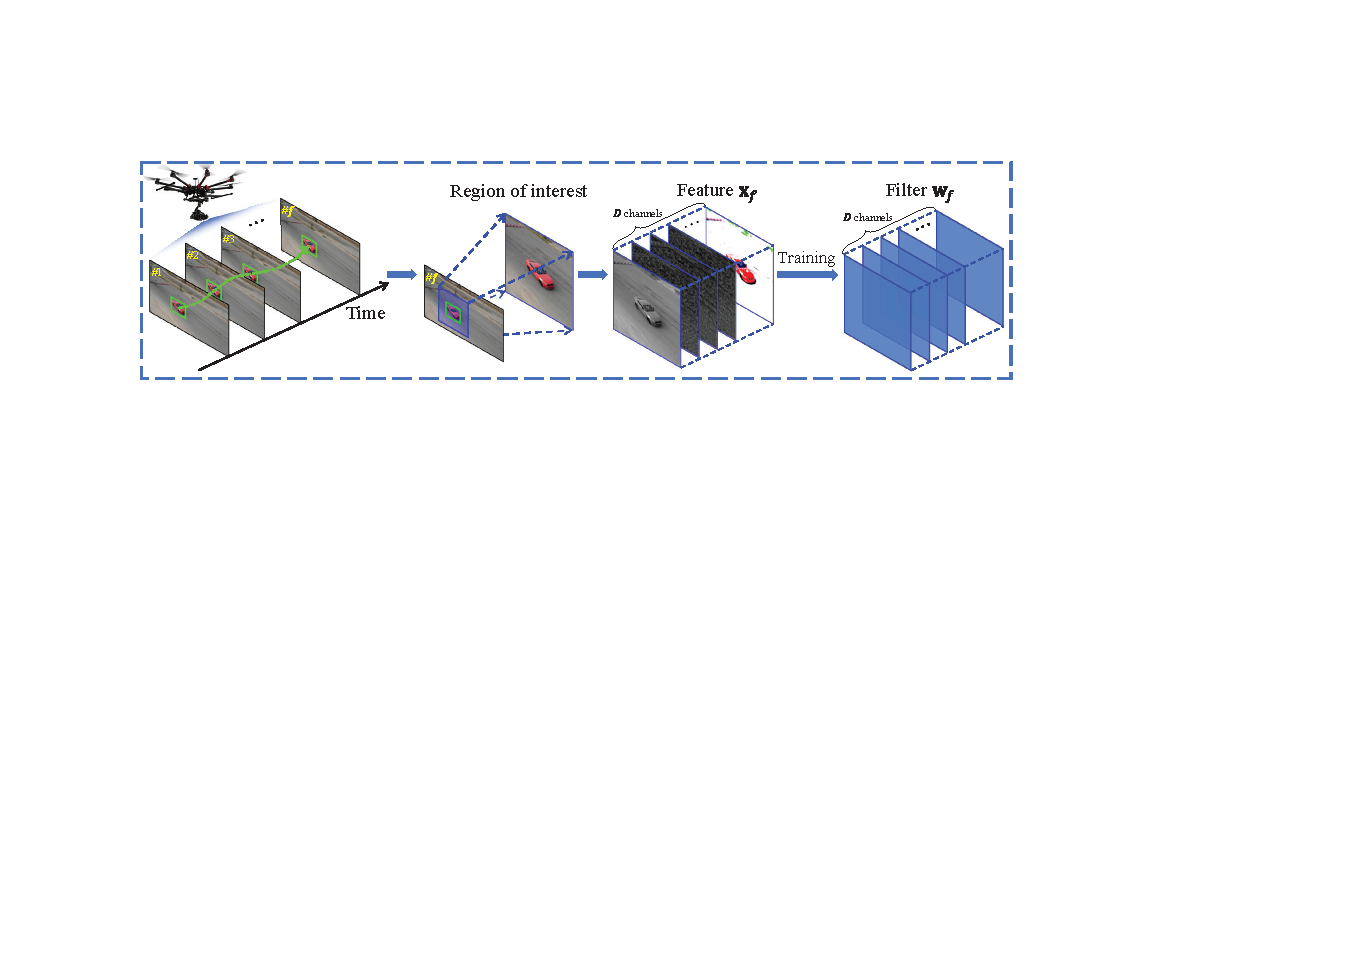
\includegraphics[width=0.7\linewidth, trim={100pt 100 100 90}]{fig/tracking_1.pdf}
        \end{center}
    \end{figure}

    which can be divided into the \textcolor{deepred}{training stage}, model update, and detection stage.

\end{frame}

\begin{frame}

    \addtocounter{footnote}{-1}
    General tracking structure of DCF-based methods onboard the UAV platform\footfullcite{fu2021correlation}:

    \begin{figure}[htpb]
        \begin{center}
            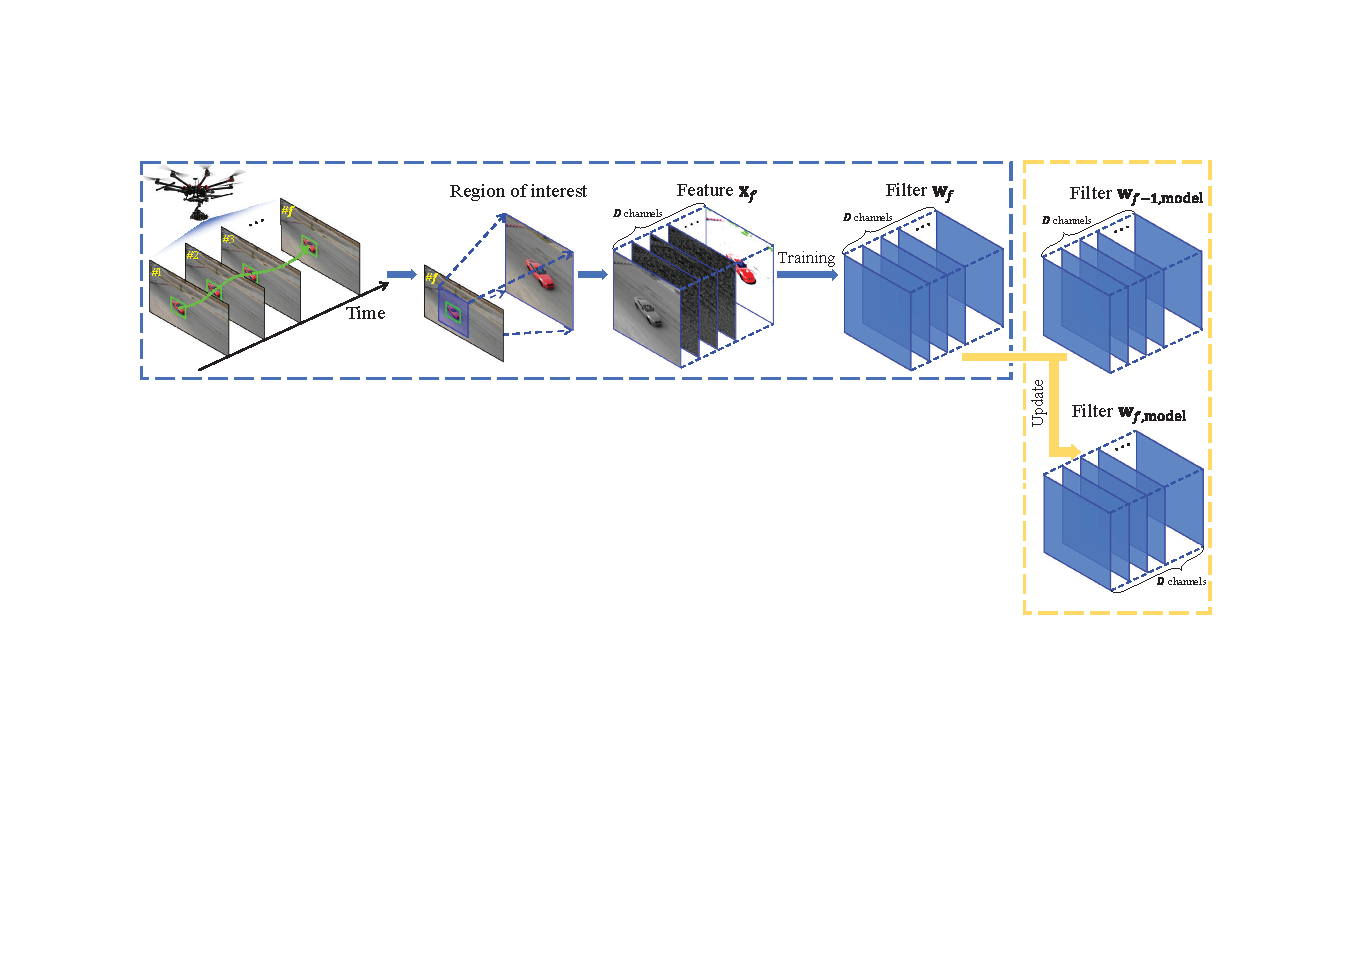
\includegraphics[width=0.7\linewidth, trim={100pt 100 100 90}]{fig/tracking_2.pdf}
        \end{center}
    \end{figure}

    which can be divided into the training stage, \textcolor{deepred}{model update}, and detection stage.

\end{frame}

\begin{frame}

    \addtocounter{footnote}{-1}
    General tracking structure of DCF-based methods onboard the UAV platform\footfullcite{fu2021correlation}:

    \begin{figure}[htpb]
        \begin{center}
            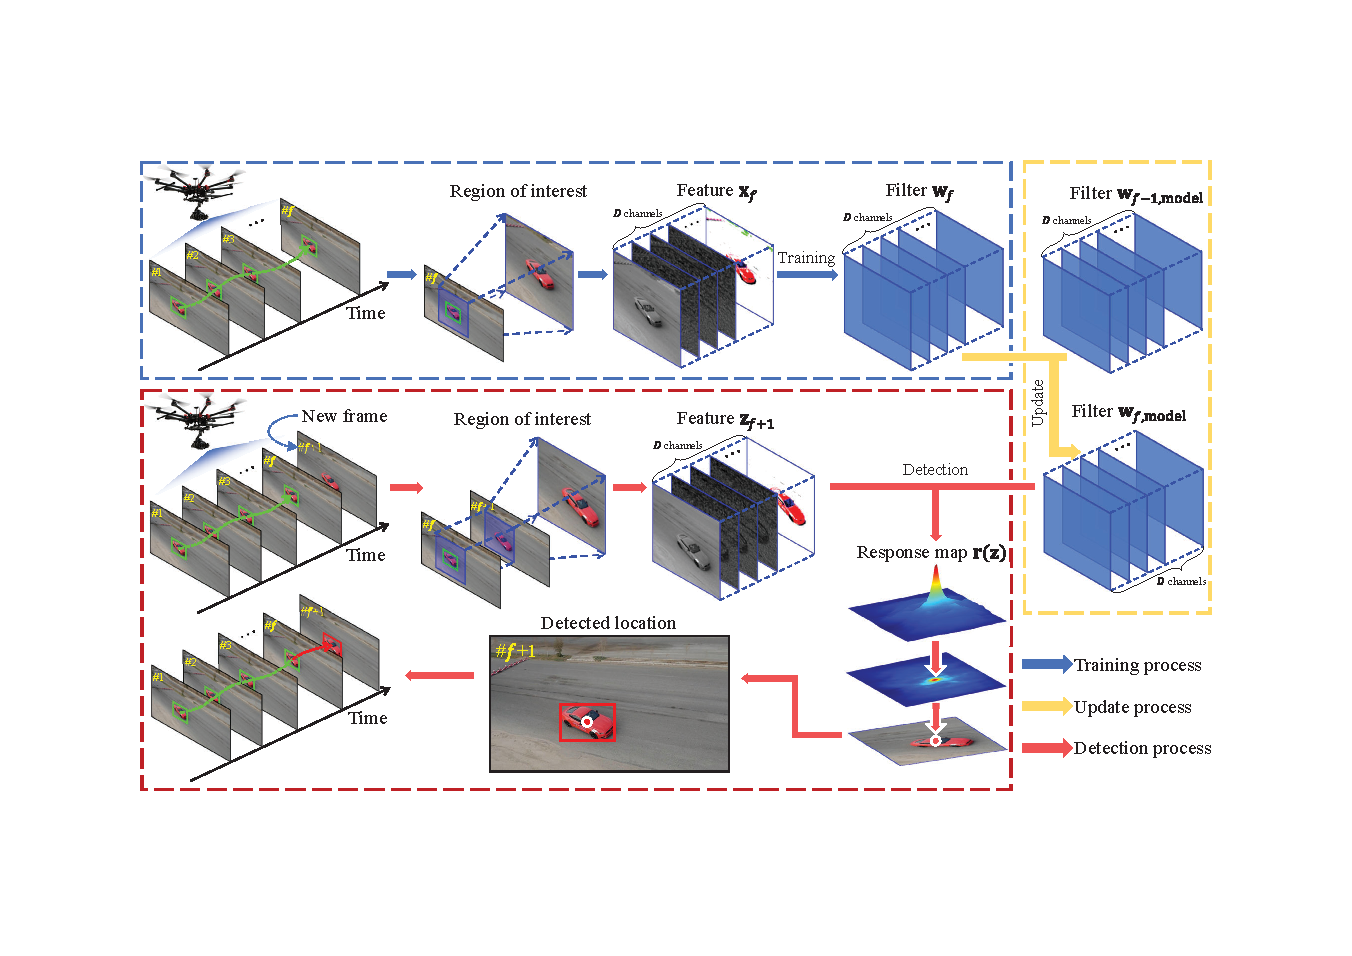
\includegraphics[width=0.7\linewidth, trim={100pt 100 100 90}]{fig/tracking_3.pdf}
        \end{center}
    \end{figure}

    which can be divided into the training stage, model update, and \textcolor{deepred}{detection stage}.

\end{frame}

\subsection{Object Tracking System}

\begin{frame}
    \begin{figure}[htpb]
        \begin{center}
            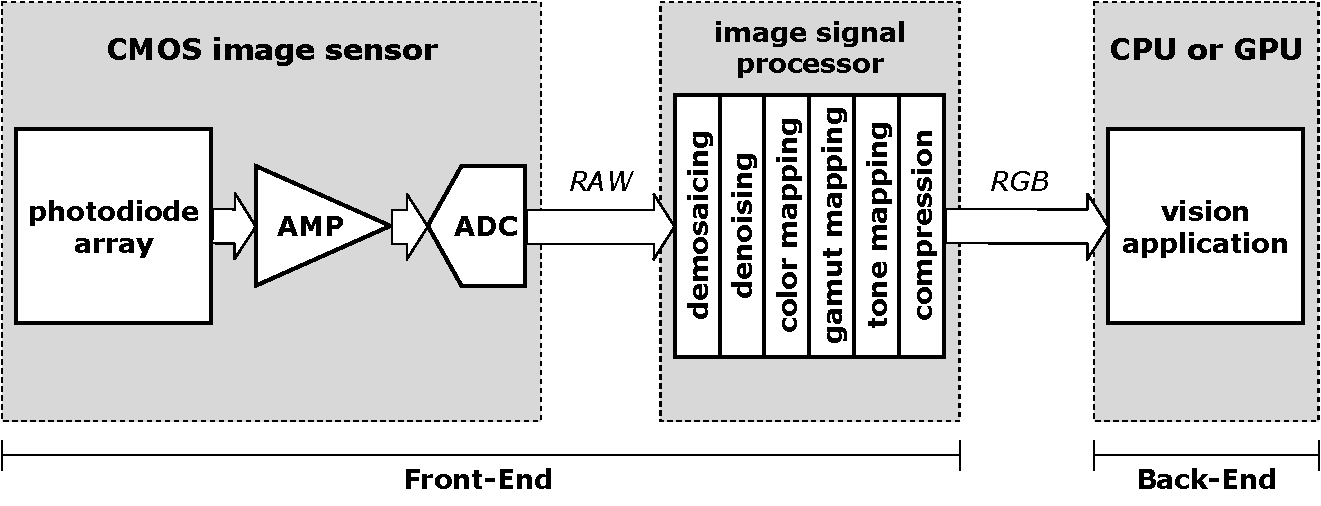
\includegraphics[width=1.0\linewidth]{fig/block.pdf}
            \caption{Object Tracking System}
        \end{center}
    \end{figure}
\end{frame}

\section{Background \& Motivation}

\section{Main Contents}

\section{Highlights}

\section{Discussion}

\begin{frame}
    \begin{center}
        {\Huge\calligra Thanks!}
    \end{center}
\end{frame}

\end{document}
